\documentclass[1p]{elsarticle_modified}
%\bibliographystyle{elsarticle-num}

%\usepackage[colorlinks]{hyperref}
%\usepackage{abbrmath_seonhwa} %\Abb, \Ascr, \Acal ,\Abf, \Afrak
\usepackage{amsfonts}
\usepackage{amssymb}
\usepackage{amsmath}
\usepackage{amsthm}
\usepackage{scalefnt}
\usepackage{amsbsy}
\usepackage{kotex}
\usepackage{caption}
\usepackage{subfig}
\usepackage{color}
\usepackage{graphicx}
\usepackage{xcolor} %% white, black, red, green, blue, cyan, magenta, yellow
\usepackage{float}
\usepackage{setspace}
\usepackage{hyperref}

\usepackage{tikz}
\usetikzlibrary{arrows}

\usepackage{multirow}
\usepackage{array} % fixed length table
\usepackage{hhline}

%%%%%%%%%%%%%%%%%%%%%
\makeatletter
\renewcommand*\env@matrix[1][\arraystretch]{%
	\edef\arraystretch{#1}%
	\hskip -\arraycolsep
	\let\@ifnextchar\new@ifnextchar
	\array{*\c@MaxMatrixCols c}}
\makeatother %https://tex.stackexchange.com/questions/14071/how-can-i-increase-the-line-spacing-in-a-matrix
%%%%%%%%%%%%%%%

\usepackage[normalem]{ulem}

\newcommand{\msout}[1]{\ifmmode\text{\sout{\ensuremath{#1}}}\else\sout{#1}\fi}
%SOURCE: \msout is \stkout macro in https://tex.stackexchange.com/questions/20609/strikeout-in-math-mode

\newcommand{\cancel}[1]{
	\ifmmode
	{\color{red}\msout{#1}}
	\else
	{\color{red}\sout{#1}}
	\fi
}

\newcommand{\add}[1]{
	{\color{blue}\uwave{#1}}
}

\newcommand{\replace}[2]{
	\ifmmode
	{\color{red}\msout{#1}}{\color{blue}\uwave{#2}}
	\else
	{\color{red}\sout{#1}}{\color{blue}\uwave{#2}}
	\fi
}

\newcommand{\Sol}{\mathcal{S}} %segment
\newcommand{\D}{D} %diagram
\newcommand{\A}{\mathcal{A}} %arc


%%%%%%%%%%%%%%%%%%%%%%%%%%%%%5 test

\def\sl{\operatorname{\textup{SL}}(2,\Cbb)}
\def\psl{\operatorname{\textup{PSL}}(2,\Cbb)}
\def\quan{\mkern 1mu \triangleright \mkern 1mu}

\theoremstyle{definition}
\newtheorem{thm}{Theorem}[section]
\newtheorem{prop}[thm]{Proposition}
\newtheorem{lem}[thm]{Lemma}
\newtheorem{ques}[thm]{Question}
\newtheorem{cor}[thm]{Corollary}
\newtheorem{defn}[thm]{Definition}
\newtheorem{exam}[thm]{Example}
\newtheorem{rmk}[thm]{Remark}
\newtheorem{alg}[thm]{Algorithm}

\newcommand{\I}{\sqrt{-1}}
\begin{document}

%\begin{frontmatter}
%
%\title{Boundary parabolic representations of knots up to 8 crossings}
%
%%% Group authors per affiliation:
%\author{Yunhi Cho} 
%\address{Department of Mathematics, University of Seoul, Seoul, Korea}
%\ead{yhcho@uos.ac.kr}
%
%
%\author{Seonhwa Kim} %\fnref{s_kim}}
%\address{Center for Geometry and Physics, Institute for Basic Science, Pohang, 37673, Korea}
%\ead{ryeona17@ibs.re.kr}
%
%\author{Hyuk Kim}
%\address{Department of Mathematical Sciences, Seoul National University, Seoul 08826, Korea}
%\ead{hyukkim@snu.ac.kr}
%
%\author{Seokbeom Yoon}
%\address{Department of Mathematical Sciences, Seoul National University, Seoul, 08826,  Korea}
%\ead{sbyoon15@snu.ac.kr}
%
%\begin{abstract}
%We find all boundary parabolic representation of knots up to 8 crossings.
%
%\end{abstract}
%\begin{keyword}
%    \MSC[2010] 57M25 
%\end{keyword}
%
%\end{frontmatter}

%\linenumbers
%\tableofcontents
%
\newcommand\colored[1]{\textcolor{white}{\rule[-0.35ex]{0.8em}{1.4ex}}\kern-0.8em\color{red} #1}%
%\newcommand\colored[1]{\textcolor{white}{ #1}\kern-2.17ex	\textcolor{white}{ #1}\kern-1.81ex	\textcolor{white}{ #1}\kern-2.15ex\color{red}#1	}

{\Large $\underline{11a_{29}~(K11a_{29})}$}

\setlength{\tabcolsep}{10pt}
\renewcommand{\arraystretch}{1.6}
\vspace{1cm}\begin{tabular}{m{100pt}>{\centering\arraybackslash}m{274pt}}
\multirow{5}{120pt}{
	\centering
	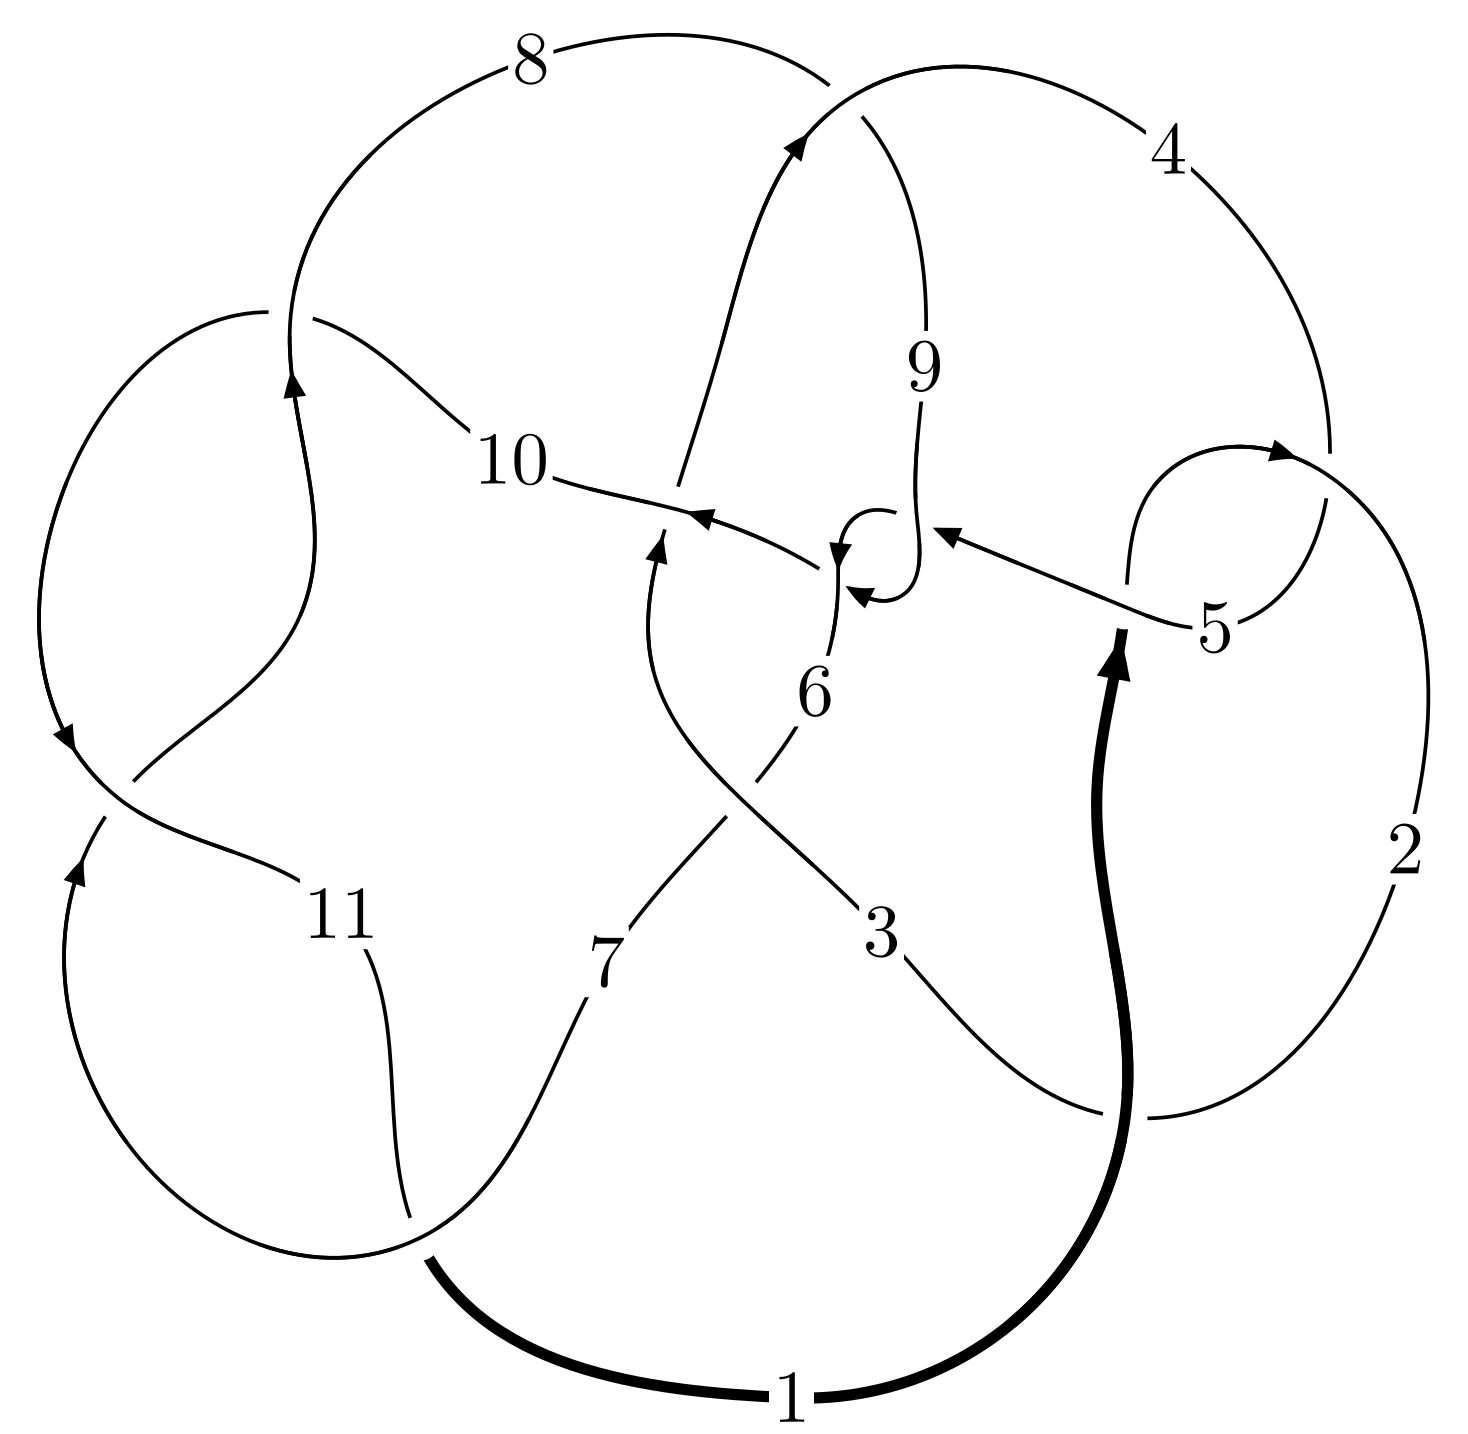
\includegraphics[width=112pt]{../../../GIT/diagram.site/Diagrams/png/278_11a_29.png}\\
\ \ \ A knot diagram\footnotemark}&
\allowdisplaybreaks
\textbf{Linearized knot diagam} \\
\cline{2-2}
 &
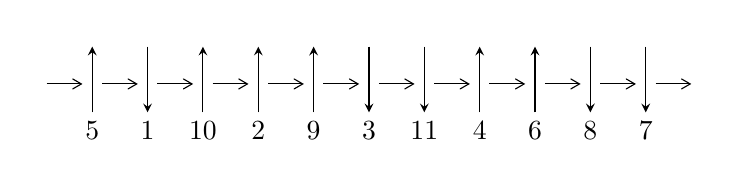
\begin{tikzpicture}[x=20pt, y=17pt]
	% nodes
	\node (C0) at (0, 0) {};
	\node (C1) at (1, 0) {};
	\node (C1U) at (1, +1) {};
	\node (C1D) at (1, -1) {5};

	\node (C2) at (2, 0) {};
	\node (C2U) at (2, +1) {};
	\node (C2D) at (2, -1) {1};

	\node (C3) at (3, 0) {};
	\node (C3U) at (3, +1) {};
	\node (C3D) at (3, -1) {10};

	\node (C4) at (4, 0) {};
	\node (C4U) at (4, +1) {};
	\node (C4D) at (4, -1) {2};

	\node (C5) at (5, 0) {};
	\node (C5U) at (5, +1) {};
	\node (C5D) at (5, -1) {9};

	\node (C6) at (6, 0) {};
	\node (C6U) at (6, +1) {};
	\node (C6D) at (6, -1) {3};

	\node (C7) at (7, 0) {};
	\node (C7U) at (7, +1) {};
	\node (C7D) at (7, -1) {11};

	\node (C8) at (8, 0) {};
	\node (C8U) at (8, +1) {};
	\node (C8D) at (8, -1) {4};

	\node (C9) at (9, 0) {};
	\node (C9U) at (9, +1) {};
	\node (C9D) at (9, -1) {6};

	\node (C10) at (10, 0) {};
	\node (C10U) at (10, +1) {};
	\node (C10D) at (10, -1) {8};

	\node (C11) at (11, 0) {};
	\node (C11U) at (11, +1) {};
	\node (C11D) at (11, -1) {7};
	\node (C12) at (12, 0) {};

	% arrows
	\draw[->,>={angle 60}]
	(C0) edge (C1) (C1) edge (C2) (C2) edge (C3) (C3) edge (C4) (C4) edge (C5) (C5) edge (C6) (C6) edge (C7) (C7) edge (C8) (C8) edge (C9) (C9) edge (C10) (C10) edge (C11) (C11) edge (C12) ;	\draw[->,>=stealth]
	(C1D) edge (C1U) (C2U) edge (C2D) (C3D) edge (C3U) (C4D) edge (C4U) (C5D) edge (C5U) (C6U) edge (C6D) (C7U) edge (C7D) (C8D) edge (C8U) (C9D) edge (C9U) (C10U) edge (C10D) (C11U) edge (C11D) ;
	\end{tikzpicture} \\
\hhline{~~} \\& 
\textbf{Solving Sequence} \\ \cline{2-2} 
 &
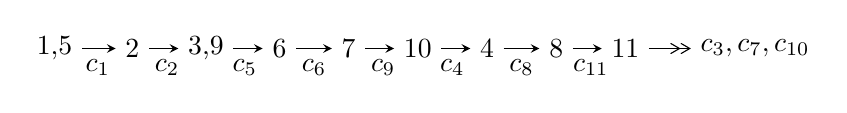
\begin{tikzpicture}[x=25pt, y=7pt]
	% node
	\node (A0) at (-1/8, 0) {1,5};
	\node (A1) at (1, 0) {2};
	\node (A2) at (33/16, 0) {3,9};
	\node (A3) at (25/8, 0) {6};
	\node (A4) at (33/8, 0) {7};
	\node (A5) at (41/8, 0) {10};
	\node (A6) at (49/8, 0) {4};
	\node (A7) at (57/8, 0) {8};
	\node (A8) at (65/8, 0) {11};
	\node (C1) at (1/2, -1) {$c_{1}$};
	\node (C2) at (3/2, -1) {$c_{2}$};
	\node (C3) at (21/8, -1) {$c_{5}$};
	\node (C4) at (29/8, -1) {$c_{6}$};
	\node (C5) at (37/8, -1) {$c_{9}$};
	\node (C6) at (45/8, -1) {$c_{4}$};
	\node (C7) at (53/8, -1) {$c_{8}$};
	\node (C8) at (61/8, -1) {$c_{11}$};
	\node (A9) at (10, 0) {$c_{3},c_{7},c_{10}$};

	% edge
	\draw[->,>=stealth]	
	(A0) edge (A1) (A1) edge (A2) (A2) edge (A3) (A3) edge (A4) (A4) edge (A5) (A5) edge (A6) (A6) edge (A7) (A7) edge (A8) ;
	\draw[->>,>={angle 60}]	
	(A8) edge (A9);
\end{tikzpicture} \\ 

\end{tabular} \\

\footnotetext{
The image of knot diagram is generated by the software ``\textbf{Draw programme}" developed by Andrew Bartholomew(\url{http://www.layer8.co.uk/maths/draw/index.htm\#Running-draw}), where we modified some parts for our purpose(\url{https://github.com/CATsTAILs/LinksPainter}).
}\phantom \\ \newline 
\centering \textbf{Ideals for irreducible components\footnotemark of $X_{\text{par}}$} 
 
\begin{align*}
I^u_{1}&=\langle 
4.99106\times10^{56} u^{60}-5.54013\times10^{56} u^{59}+\cdots+3.76009\times10^{57} b-3.71146\times10^{57},\\
\phantom{I^u_{1}}&\phantom{= \langle  }-3.10364\times10^{57} u^{60}+5.28988\times10^{57} u^{59}+\cdots+1.12803\times10^{58} a-3.91838\times10^{58},\;u^{61}-3 u^{60}+\cdots-5 u+9\rangle \\
I^u_{2}&=\langle 
3 b+2 u-2,\;a+1,\;u^2+u+1\rangle \\
I^u_{3}&=\langle 
3 b-2 u-1,\;a+u,\;u^2+u+1\rangle \\
\\
\end{align*}
\raggedright * 3 irreducible components of $\dim_{\mathbb{C}}=0$, with total 65 representations.\\
\footnotetext{All coefficients of polynomials are rational numbers. But the coefficients are sometimes approximated in decimal forms when there is not enough margin.}
\newpage
\renewcommand{\arraystretch}{1}
\centering \section*{I. $I^u_{1}= \langle 4.99\times10^{56} u^{60}-5.54\times10^{56} u^{59}+\cdots+3.76\times10^{57} b-3.71\times10^{57},\;-3.10\times10^{57} u^{60}+5.29\times10^{57} u^{59}+\cdots+1.13\times10^{58} a-3.92\times10^{58},\;u^{61}-3 u^{60}+\cdots-5 u+9 \rangle$}
\flushleft \textbf{(i) Arc colorings}\\
\begin{tabular}{m{7pt} m{180pt} m{7pt} m{180pt} }
\flushright $a_{1}=$&$\begin{pmatrix}1\\0\end{pmatrix}$ \\
\flushright $a_{5}=$&$\begin{pmatrix}0\\u\end{pmatrix}$ \\
\flushright $a_{2}=$&$\begin{pmatrix}1\\- u^2\end{pmatrix}$ \\
\flushright $a_{3}=$&$\begin{pmatrix}u^2+1\\- u^2\end{pmatrix}$ \\
\flushright $a_{9}=$&$\begin{pmatrix}0.275139 u^{60}-0.468950 u^{59}+\cdots+4.47285 u+3.47366\\-0.132738 u^{60}+0.147340 u^{59}+\cdots-4.15830 u+0.987068\end{pmatrix}$ \\
\flushright $a_{6}=$&$\begin{pmatrix}1.11106 u^{60}-2.61700 u^{59}+\cdots+5.79571 u-5.77693\\-0.595122 u^{60}+2.16473 u^{59}+\cdots+2.14031 u+12.7347\end{pmatrix}$ \\
\flushright $a_{7}=$&$\begin{pmatrix}0.302897 u^{60}-0.758393 u^{59}+\cdots+2.22294 u-1.51536\\-0.161015 u^{60}+0.635343 u^{59}+\cdots+2.73852 u+5.59822\end{pmatrix}$ \\
\flushright $a_{10}=$&$\begin{pmatrix}0.327154 u^{60}-0.474281 u^{59}+\cdots+10.9343 u+2.92153\\-0.507182 u^{60}+1.24714 u^{59}+\cdots-4.55730 u+2.94439\end{pmatrix}$ \\
\flushright $a_{4}=$&$\begin{pmatrix}- u\\u^3+u\end{pmatrix}$ \\
\flushright $a_{8}=$&$\begin{pmatrix}0.849189 u^{60}-1.82096 u^{59}+\cdots+7.07757 u+2.72833\\-0.575418 u^{60}+1.58164 u^{59}+\cdots-3.44728 u+5.06368\end{pmatrix}$ \\
\flushright $a_{11}=$&$\begin{pmatrix}-0.289728 u^{60}+0.616900 u^{59}+\cdots+6.66475 u+2.26231\\0.0110587 u^{60}-0.250053 u^{59}+\cdots-0.805308 u-1.89157\end{pmatrix}$\\ \flushright $a_{11}=$&$\begin{pmatrix}-0.289728 u^{60}+0.616900 u^{59}+\cdots+6.66475 u+2.26231\\0.0110587 u^{60}-0.250053 u^{59}+\cdots-0.805308 u-1.89157\end{pmatrix}$\\&\end{tabular}
\flushleft \textbf{(ii) Obstruction class $= -1$}\\~\\
\flushleft \textbf{(iii) Cusp Shapes $= 1.51281 u^{60}-3.43786 u^{59}+\cdots+30.9340 u-2.78257$}\\~\\
\newpage\renewcommand{\arraystretch}{1}
\flushleft \textbf{(iv) u-Polynomials at the component}\newline \\
\begin{tabular}{m{50pt}|m{274pt}}
Crossings & \hspace{64pt}u-Polynomials at each crossing \\
\hline $$\begin{aligned}c_{1},c_{4}\end{aligned}$$&$\begin{aligned}
&u^{61}+3 u^{60}+\cdots-5 u-9
\end{aligned}$\\
\hline $$\begin{aligned}c_{2}\end{aligned}$$&$\begin{aligned}
&u^{61}+21 u^{60}+\cdots-1505 u-81
\end{aligned}$\\
\hline $$\begin{aligned}c_{3}\end{aligned}$$&$\begin{aligned}
&u^{61}-3 u^{60}+\cdots-1872 u+432
\end{aligned}$\\
\hline $$\begin{aligned}c_{5},c_{9}\end{aligned}$$&$\begin{aligned}
&u^{61}-3 u^{60}+\cdots+3 u-1
\end{aligned}$\\
\hline $$\begin{aligned}c_{6}\end{aligned}$$&$\begin{aligned}
&9(9 u^{61}-30 u^{60}+\cdots+293350 u-68375)
\end{aligned}$\\
\hline $$\begin{aligned}c_{7},c_{10},c_{11}\end{aligned}$$&$\begin{aligned}
&u^{61}-3 u^{60}+\cdots+3 u-1
\end{aligned}$\\
\hline $$\begin{aligned}c_{8}\end{aligned}$$&$\begin{aligned}
&9(9 u^{61}+57 u^{60}+\cdots-10059 u-2801)
\end{aligned}$\\
\hline
\end{tabular}\\~\\
\newpage\renewcommand{\arraystretch}{1}
\flushleft \textbf{(v) Riley Polynomials at the component}\newline \\
\begin{tabular}{m{50pt}|m{274pt}}
Crossings & \hspace{64pt}Riley Polynomials at each crossing \\
\hline $$\begin{aligned}c_{1},c_{4}\end{aligned}$$&$\begin{aligned}
&y^{61}+21 y^{60}+\cdots-1505 y-81
\end{aligned}$\\
\hline $$\begin{aligned}c_{2}\end{aligned}$$&$\begin{aligned}
&y^{61}+41 y^{60}+\cdots+37363 y-6561
\end{aligned}$\\
\hline $$\begin{aligned}c_{3}\end{aligned}$$&$\begin{aligned}
&y^{61}-25 y^{60}+\cdots+1897344 y-186624
\end{aligned}$\\
\hline $$\begin{aligned}c_{5},c_{9}\end{aligned}$$&$\begin{aligned}
&y^{61}-39 y^{60}+\cdots-13 y-1
\end{aligned}$\\
\hline $$\begin{aligned}c_{6}\end{aligned}$$&$\begin{aligned}
&81(81 y^{61}+3546 y^{60}+\cdots-9.00135\times10^{10} y-4.67514\times10^{9})
\end{aligned}$\\
\hline $$\begin{aligned}c_{7},c_{10},c_{11}\end{aligned}$$&$\begin{aligned}
&y^{61}+61 y^{60}+\cdots-13 y-1
\end{aligned}$\\
\hline $$\begin{aligned}c_{8}\end{aligned}$$&$\begin{aligned}
&81(81 y^{61}-2259 y^{60}+\cdots+1.36190\times10^{8} y-7845601)
\end{aligned}$\\
\hline
\end{tabular}\\~\\
\newpage\flushleft \textbf{(vi) Complex Volumes and Cusp Shapes}
$$\begin{array}{c|c|c}  
\text{Solutions to }I^u_{1}& \I (\text{vol} + \sqrt{-1}CS) & \text{Cusp shape}\\
 \hline 
\begin{aligned}
u &= \phantom{-}0.627295 + 0.781178 I \\
a &= \phantom{-}0.779915 + 0.938460 I \\
b &= -0.133545 - 0.868985 I\end{aligned}
 & \phantom{-}0.680796 - 0.488788 I & \phantom{-}8.37952 + 2.33314 I \\ \hline\begin{aligned}
u &= \phantom{-}0.627295 - 0.781178 I \\
a &= \phantom{-}0.779915 - 0.938460 I \\
b &= -0.133545 + 0.868985 I\end{aligned}
 & \phantom{-}0.680796 + 0.488788 I & \phantom{-}8.37952 - 2.33314 I \\ \hline\begin{aligned}
u &= -0.909616 + 0.468593 I \\
a &= -1.059460 - 0.502224 I \\
b &= \phantom{-}1.43290 - 0.75784 I\end{aligned}
 & \phantom{-}4.73566 - 1.67644 I & \phantom{-}12.36420 + 3.79278 I \\ \hline\begin{aligned}
u &= -0.909616 - 0.468593 I \\
a &= -1.059460 + 0.502224 I \\
b &= \phantom{-}1.43290 + 0.75784 I\end{aligned}
 & \phantom{-}4.73566 + 1.67644 I & \phantom{-}12.36420 - 3.79278 I \\ \hline\begin{aligned}
u &= \phantom{-}0.823832 + 0.641756 I \\
a &= -0.493457 - 0.867597 I \\
b &= \phantom{-}0.171205 + 0.613586 I\end{aligned}
 & \phantom{-}8.40390 - 4.08328 I & \phantom{-}6.32782 + 2.17005 I \\ \hline\begin{aligned}
u &= \phantom{-}0.823832 - 0.641756 I \\
a &= -0.493457 + 0.867597 I \\
b &= \phantom{-}0.171205 - 0.613586 I\end{aligned}
 & \phantom{-}8.40390 + 4.08328 I & \phantom{-}6.32782 - 2.17005 I \\ \hline\begin{aligned}
u &= \phantom{-}0.084826 + 0.951096 I \\
a &= \phantom{-}0.768701 - 0.355562 I \\
b &= -0.926574 - 0.590119 I\end{aligned}
 & -3.04092 - 0.55487 I & -5.63926 + 1.54785 I \\ \hline\begin{aligned}
u &= \phantom{-}0.084826 - 0.951096 I \\
a &= \phantom{-}0.768701 + 0.355562 I \\
b &= -0.926574 + 0.590119 I\end{aligned}
 & -3.04092 + 0.55487 I & -5.63926 - 1.54785 I \\ \hline\begin{aligned}
u &= \phantom{-}0.745313 + 0.734834 I \\
a &= -0.69455 + 1.28009 I \\
b &= \phantom{-}1.59810 + 0.54771 I\end{aligned}
 & \phantom{-}5.33189 - 0.62357 I & \phantom{-}6.90078 + 0. I\phantom{ +0.000000I} \\ \hline\begin{aligned}
u &= \phantom{-}0.745313 - 0.734834 I \\
a &= -0.69455 - 1.28009 I \\
b &= \phantom{-}1.59810 - 0.54771 I\end{aligned}
 & \phantom{-}5.33189 + 0.62357 I & \phantom{-}6.90078 + 0. I\phantom{ +0.000000I}\\
 \hline 
 \end{array}$$\newpage$$\begin{array}{c|c|c}  
\text{Solutions to }I^u_{1}& \I (\text{vol} + \sqrt{-1}CS) & \text{Cusp shape}\\
 \hline 
\begin{aligned}
u &= -0.592571 + 0.868966 I \\
a &= \phantom{-}0.643580 + 0.821069 I \\
b &= -3.23298 + 1.50658 I\end{aligned}
 & \phantom{-}2.11702 - 2.33942 I & -10.06681 - 7.06956 I \\ \hline\begin{aligned}
u &= -0.592571 - 0.868966 I \\
a &= \phantom{-}0.643580 - 0.821069 I \\
b &= -3.23298 - 1.50658 I\end{aligned}
 & \phantom{-}2.11702 + 2.33942 I & -10.06681 + 7.06956 I \\ \hline\begin{aligned}
u &= \phantom{-}0.869096 + 0.612382 I \\
a &= \phantom{-}0.840207 - 1.089160 I \\
b &= -1.66751 - 0.62148 I\end{aligned}
 & \phantom{-}5.98865 - 5.78069 I & \phantom{-}6.25624 + 4.52312 I \\ \hline\begin{aligned}
u &= \phantom{-}0.869096 - 0.612382 I \\
a &= \phantom{-}0.840207 + 1.089160 I \\
b &= -1.66751 + 0.62148 I\end{aligned}
 & \phantom{-}5.98865 + 5.78069 I & \phantom{-}6.25624 - 4.52312 I \\ \hline\begin{aligned}
u &= -0.510457 + 0.948104 I \\
a &= \phantom{-}0.221723 - 0.095163 I \\
b &= -0.197711 - 0.400616 I\end{aligned}
 & -0.17638 - 2.59422 I & \phantom{-0.000000 } 0 \\ \hline\begin{aligned}
u &= -0.510457 - 0.948104 I \\
a &= \phantom{-}0.221723 + 0.095163 I \\
b &= -0.197711 + 0.400616 I\end{aligned}
 & -0.17638 + 2.59422 I & \phantom{-0.000000 } 0 \\ \hline\begin{aligned}
u &= \phantom{-}0.642563 + 0.936820 I \\
a &= -0.882906 - 0.630814 I \\
b &= \phantom{-}0.433541 + 0.916219 I\end{aligned}
 & \phantom{-}0.17275 + 5.47510 I & \phantom{-0.000000 } 0 \\ \hline\begin{aligned}
u &= \phantom{-}0.642563 - 0.936820 I \\
a &= -0.882906 + 0.630814 I \\
b &= \phantom{-}0.433541 - 0.916219 I\end{aligned}
 & \phantom{-}0.17275 - 5.47510 I & \phantom{-0.000000 } 0 \\ \hline\begin{aligned}
u &= \phantom{-}0.318467 + 0.797607 I \\
a &= -1.256550 + 0.401471 I \\
b &= \phantom{-}1.24853 + 0.72368 I\end{aligned}
 & -0.53178 + 3.55128 I & -1.97116 + 0.53822 I \\ \hline\begin{aligned}
u &= \phantom{-}0.318467 - 0.797607 I \\
a &= -1.256550 - 0.401471 I \\
b &= \phantom{-}1.24853 - 0.72368 I\end{aligned}
 & -0.53178 - 3.55128 I & -1.97116 - 0.53822 I\\
 \hline 
 \end{array}$$\newpage$$\begin{array}{c|c|c}  
\text{Solutions to }I^u_{1}& \I (\text{vol} + \sqrt{-1}CS) & \text{Cusp shape}\\
 \hline 
\begin{aligned}
u &= -0.541792 + 0.666328 I \\
a &= -0.443464 - 0.720747 I \\
b &= -1.80634 + 0.47653 I\end{aligned}
 & \phantom{-}6.77383 - 1.39600 I & \phantom{-}1.94563 + 3.09396 I \\ \hline\begin{aligned}
u &= -0.541792 - 0.666328 I \\
a &= -0.443464 + 0.720747 I \\
b &= -1.80634 - 0.47653 I\end{aligned}
 & \phantom{-}6.77383 + 1.39600 I & \phantom{-}1.94563 - 3.09396 I \\ \hline\begin{aligned}
u &= -0.105247 + 1.136650 I \\
a &= -0.528868 + 0.217428 I \\
b &= \phantom{-}0.733637 + 0.607458 I\end{aligned}
 & \phantom{-}1.89473 - 3.39241 I & \phantom{-0.000000 } 0 \\ \hline\begin{aligned}
u &= -0.105247 - 1.136650 I \\
a &= -0.528868 - 0.217428 I \\
b &= \phantom{-}0.733637 - 0.607458 I\end{aligned}
 & \phantom{-}1.89473 + 3.39241 I & \phantom{-0.000000 } 0 \\ \hline\begin{aligned}
u &= -0.430215 + 0.742658 I \\
a &= \phantom{-}0.120777 + 0.430167 I \\
b &= \phantom{-}0.656197 - 0.151023 I\end{aligned}
 & \phantom{-}0.53014 - 1.40693 I & \phantom{-}5.62347 + 5.20497 I \\ \hline\begin{aligned}
u &= -0.430215 - 0.742658 I \\
a &= \phantom{-}0.120777 - 0.430167 I \\
b &= \phantom{-}0.656197 + 0.151023 I\end{aligned}
 & \phantom{-}0.53014 + 1.40693 I & \phantom{-}5.62347 - 5.20497 I \\ \hline\begin{aligned}
u &= \phantom{-}0.769003 + 0.845851 I \\
a &= \phantom{-}1.196660 - 0.497619 I \\
b &= -2.31477 - 0.56610 I\end{aligned}
 & \phantom{-}11.92950 + 1.96301 I & \phantom{-0.000000 } 0 \\ \hline\begin{aligned}
u &= \phantom{-}0.769003 - 0.845851 I \\
a &= \phantom{-}1.196660 + 0.497619 I \\
b &= -2.31477 + 0.56610 I\end{aligned}
 & \phantom{-}11.92950 - 1.96301 I & \phantom{-0.000000 } 0 \\ \hline\begin{aligned}
u &= -0.035967 + 0.854814 I \\
a &= \phantom{-}0.563353 + 0.959661 I \\
b &= -0.057385 - 0.568156 I\end{aligned}
 & \phantom{-}0.13425 - 1.52358 I & \phantom{-}1.52672 + 2.12846 I \\ \hline\begin{aligned}
u &= -0.035967 - 0.854814 I \\
a &= \phantom{-}0.563353 - 0.959661 I \\
b &= -0.057385 + 0.568156 I\end{aligned}
 & \phantom{-}0.13425 + 1.52358 I & \phantom{-}1.52672 - 2.12846 I\\
 \hline 
 \end{array}$$\newpage$$\begin{array}{c|c|c}  
\text{Solutions to }I^u_{1}& \I (\text{vol} + \sqrt{-1}CS) & \text{Cusp shape}\\
 \hline 
\begin{aligned}
u &= \phantom{-}0.757313 + 0.895285 I \\
a &= \phantom{-}0.456980 - 1.227760 I \\
b &= -1.41876 - 0.53071 I\end{aligned}
 & \phantom{-}11.77860 + 3.79247 I & \phantom{-0.000000 } 0 \\ \hline\begin{aligned}
u &= \phantom{-}0.757313 - 0.895285 I \\
a &= \phantom{-}0.456980 + 1.227760 I \\
b &= -1.41876 + 0.53071 I\end{aligned}
 & \phantom{-}11.77860 - 3.79247 I & \phantom{-0.000000 } 0 \\ \hline\begin{aligned}
u &= \phantom{-}1.008640 + 0.609371 I \\
a &= -0.801725 + 0.933371 I \\
b &= \phantom{-}1.70920 + 0.69780 I\end{aligned}
 & \phantom{-}13.1909 - 9.2873 I & \phantom{-0.000000 } 0 \\ \hline\begin{aligned}
u &= \phantom{-}1.008640 - 0.609371 I \\
a &= -0.801725 - 0.933371 I \\
b &= \phantom{-}1.70920 - 0.69780 I\end{aligned}
 & \phantom{-}13.1909 + 9.2873 I & \phantom{-0.000000 } 0 \\ \hline\begin{aligned}
u &= \phantom{-}0.699249 + 0.967906 I \\
a &= -1.098020 + 0.664109 I \\
b &= \phantom{-}2.41658 + 0.73364 I\end{aligned}
 & \phantom{-}4.62247 + 6.13062 I & \phantom{-0.000000 } 0 \\ \hline\begin{aligned}
u &= \phantom{-}0.699249 - 0.967906 I \\
a &= -1.098020 - 0.664109 I \\
b &= \phantom{-}2.41658 - 0.73364 I\end{aligned}
 & \phantom{-}4.62247 - 6.13062 I & \phantom{-0.000000 } 0 \\ \hline\begin{aligned}
u &= -0.312667 + 0.736573 I \\
a &= -0.52054 - 1.36729 I \\
b &= -0.76632 - 2.47025 I\end{aligned}
 & \phantom{-}6.16730 - 1.44795 I & \phantom{-}6.66665 + 4.19132 I \\ \hline\begin{aligned}
u &= -0.312667 - 0.736573 I \\
a &= -0.52054 + 1.36729 I \\
b &= -0.76632 + 2.47025 I\end{aligned}
 & \phantom{-}6.16730 + 1.44795 I & \phantom{-}6.66665 - 4.19132 I \\ \hline\begin{aligned}
u &= -0.141017 + 1.196910 I \\
a &= -0.409903 - 0.838432 I \\
b &= \phantom{-}0.617600 + 0.023876 I\end{aligned}
 & -1.00556 - 4.64477 I & \phantom{-0.000000 } 0 \\ \hline\begin{aligned}
u &= -0.141017 - 1.196910 I \\
a &= -0.409903 + 0.838432 I \\
b &= \phantom{-}0.617600 - 0.023876 I\end{aligned}
 & -1.00556 + 4.64477 I & \phantom{-0.000000 } 0\\
 \hline 
 \end{array}$$\newpage$$\begin{array}{c|c|c}  
\text{Solutions to }I^u_{1}& \I (\text{vol} + \sqrt{-1}CS) & \text{Cusp shape}\\
 \hline 
\begin{aligned}
u &= -0.657124 + 1.017530 I \\
a &= -0.322773 + 0.051413 I \\
b &= \phantom{-}0.113526 + 0.695926 I\end{aligned}
 & \phantom{-}5.54533 - 3.61915 I & \phantom{-0.000000 } 0 \\ \hline\begin{aligned}
u &= -0.657124 - 1.017530 I \\
a &= -0.322773 - 0.051413 I \\
b &= \phantom{-}0.113526 - 0.695926 I\end{aligned}
 & \phantom{-}5.54533 + 3.61915 I & \phantom{-0.000000 } 0 \\ \hline\begin{aligned}
u &= \phantom{-}0.711728 + 1.036980 I \\
a &= \phantom{-}0.745027 + 0.504667 I \\
b &= -0.521745 - 0.778989 I\end{aligned}
 & \phantom{-}7.21133 + 9.84159 I & \phantom{-0.000000 } 0 \\ \hline\begin{aligned}
u &= \phantom{-}0.711728 - 1.036980 I \\
a &= \phantom{-}0.745027 - 0.504667 I \\
b &= -0.521745 + 0.778989 I\end{aligned}
 & \phantom{-}7.21133 - 9.84159 I & \phantom{-0.000000 } 0 \\ \hline\begin{aligned}
u &= -0.602854 + 0.415244 I \\
a &= -0.754289 - 0.133208 I \\
b &= -0.631853 + 0.712874 I\end{aligned}
 & \phantom{-}6.86257 - 1.40524 I & \phantom{-}4.78353 + 3.77219 I \\ \hline\begin{aligned}
u &= -0.602854 - 0.415244 I \\
a &= -0.754289 + 0.133208 I \\
b &= -0.631853 - 0.712874 I\end{aligned}
 & \phantom{-}6.86257 + 1.40524 I & \phantom{-}4.78353 - 3.77219 I \\ \hline\begin{aligned}
u &= \phantom{-}0.717435 + 1.062890 I \\
a &= \phantom{-}0.966509 - 0.663460 I \\
b &= -2.53101 - 0.75950 I\end{aligned}
 & \phantom{-}4.62032 + 11.67140 I & \phantom{-0.000000 } 0 \\ \hline\begin{aligned}
u &= \phantom{-}0.717435 - 1.062890 I \\
a &= \phantom{-}0.966509 + 0.663460 I \\
b &= -2.53101 + 0.75950 I\end{aligned}
 & \phantom{-}4.62032 - 11.67140 I & \phantom{-0.000000 } 0 \\ \hline\begin{aligned}
u &= -0.736476 + 1.080940 I \\
a &= -0.590572 - 0.661323 I \\
b &= \phantom{-}2.05889 - 0.64346 I\end{aligned}
 & \phantom{-}2.98645 - 4.33485 I & \phantom{-0.000000 } 0 \\ \hline\begin{aligned}
u &= -0.736476 - 1.080940 I \\
a &= -0.590572 + 0.661323 I \\
b &= \phantom{-}2.05889 + 0.64346 I\end{aligned}
 & \phantom{-}2.98645 + 4.33485 I & \phantom{-0.000000 } 0\\
 \hline 
 \end{array}$$\newpage$$\begin{array}{c|c|c}  
\text{Solutions to }I^u_{1}& \I (\text{vol} + \sqrt{-1}CS) & \text{Cusp shape}\\
 \hline 
\begin{aligned}
u &= \phantom{-}0.762794 + 1.122440 I \\
a &= -0.897935 + 0.616455 I \\
b &= \phantom{-}2.61369 + 0.74270 I\end{aligned}
 & \phantom{-}11.5735 + 15.7181 I & \phantom{-0.000000 } 0 \\ \hline\begin{aligned}
u &= \phantom{-}0.762794 - 1.122440 I \\
a &= -0.897935 - 0.616455 I \\
b &= \phantom{-}2.61369 - 0.74270 I\end{aligned}
 & \phantom{-}11.5735 - 15.7181 I & \phantom{-0.000000 } 0 \\ \hline\begin{aligned}
u &= -1.265180 + 0.491129 I \\
a &= \phantom{-}0.862536 + 0.296472 I \\
b &= -1.81507 + 0.52494 I\end{aligned}
 & \phantom{-}11.53690 - 2.05353 I & \phantom{-0.000000 } 0 \\ \hline\begin{aligned}
u &= -1.265180 - 0.491129 I \\
a &= \phantom{-}0.862536 - 0.296472 I \\
b &= -1.81507 - 0.52494 I\end{aligned}
 & \phantom{-}11.53690 + 2.05353 I & \phantom{-0.000000 } 0 \\ \hline\begin{aligned}
u &= -0.23194 + 1.39578 I \\
a &= \phantom{-}0.368146 + 0.755457 I \\
b &= -0.844858 + 0.405684 I\end{aligned}
 & \phantom{-}4.72211 - 7.08106 I & \phantom{-0.000000 } 0 \\ \hline\begin{aligned}
u &= -0.23194 - 1.39578 I \\
a &= \phantom{-}0.368146 - 0.755457 I \\
b &= -0.844858 - 0.405684 I\end{aligned}
 & \phantom{-}4.72211 + 7.08106 I & \phantom{-0.000000 } 0 \\ \hline\begin{aligned}
u &= -0.91950 + 1.21328 I \\
a &= \phantom{-}0.561522 + 0.564425 I \\
b &= -1.88530 + 0.80608 I\end{aligned}
 & \phantom{-}9.38339 - 5.57107 I & \phantom{-0.000000 } 0 \\ \hline\begin{aligned}
u &= -0.91950 - 1.21328 I \\
a &= \phantom{-}0.561522 - 0.564425 I \\
b &= -1.88530 - 0.80608 I\end{aligned}
 & \phantom{-}9.38339 + 5.57107 I & \phantom{-0.000000 } 0 \\ \hline\begin{aligned}
u &= -0.408049\phantom{ +0.000000I} \\
a &= \phantom{-}2.87652\phantom{ +0.000000I} \\
b &= -0.0942688\phantom{ +0.000000I}\end{aligned}
 & \phantom{-}2.58372\phantom{ +0.000000I} & \phantom{-}0.156380\phantom{ +0.000000I} \\ \hline\begin{aligned}
u &= \phantom{-}0.159087 + 0.350060 I \\
a &= \phantom{-}0.83224 + 1.41611 I \\
b &= \phantom{-}0.161959 - 0.489660 I\end{aligned}
 & \phantom{-}0.145306 - 1.198500 I & \phantom{-}1.41714 + 6.05642 I\\
 \hline 
 \end{array}$$\newpage$$\begin{array}{c|c|c}  
\text{Solutions to }I^u_{1}& \I (\text{vol} + \sqrt{-1}CS) & \text{Cusp shape}\\
 \hline 
\begin{aligned}
u &= \phantom{-}0.159087 - 0.350060 I \\
a &= \phantom{-}0.83224 - 1.41611 I \\
b &= \phantom{-}0.161959 + 0.489660 I\end{aligned}
 & \phantom{-}0.145306 + 1.198500 I & \phantom{-}1.41714 - 6.05642 I\\
 \hline 
 \end{array}$$\newpage\newpage\renewcommand{\arraystretch}{1}
\centering \section*{II. $I^u_{2}= \langle 3 b+2 u-2,\;a+1,\;u^2+u+1 \rangle$}
\flushleft \textbf{(i) Arc colorings}\\
\begin{tabular}{m{7pt} m{180pt} m{7pt} m{180pt} }
\flushright $a_{1}=$&$\begin{pmatrix}1\\0\end{pmatrix}$ \\
\flushright $a_{5}=$&$\begin{pmatrix}0\\u\end{pmatrix}$ \\
\flushright $a_{2}=$&$\begin{pmatrix}1\\u+1\end{pmatrix}$ \\
\flushright $a_{3}=$&$\begin{pmatrix}- u\\u+1\end{pmatrix}$ \\
\flushright $a_{9}=$&$\begin{pmatrix}-1\\-\frac{2}{3} u+\frac{2}{3}\end{pmatrix}$ \\
\flushright $a_{6}=$&$\begin{pmatrix}u\\-\frac{1}{3} u-\frac{2}{3}\end{pmatrix}$ \\
\flushright $a_{7}=$&$\begin{pmatrix}\frac{4}{3} u-\frac{1}{3}\\- u-1\end{pmatrix}$ \\
\flushright $a_{10}=$&$\begin{pmatrix}- u-2\\- u+1\end{pmatrix}$ \\
\flushright $a_{4}=$&$\begin{pmatrix}- u\\u+1\end{pmatrix}$ \\
\flushright $a_{8}=$&$\begin{pmatrix}\frac{2}{3} u-\frac{2}{3}\\- u\end{pmatrix}$ \\
\flushright $a_{11}=$&$\begin{pmatrix}-\frac{1}{3} u-\frac{2}{3}\\- u\end{pmatrix}$\\ \flushright $a_{11}=$&$\begin{pmatrix}-\frac{1}{3} u-\frac{2}{3}\\- u\end{pmatrix}$\\&\end{tabular}
\flushleft \textbf{(ii) Obstruction class $= 1$}\\~\\
\flushleft \textbf{(iii) Cusp Shapes $= 8 u+\frac{28}{3}$}\\~\\
\newpage\renewcommand{\arraystretch}{1}
\flushleft \textbf{(iv) u-Polynomials at the component}\newline \\
\begin{tabular}{m{50pt}|m{274pt}}
Crossings & \hspace{64pt}u-Polynomials at each crossing \\
\hline $$\begin{aligned}c_{1},c_{2},c_{5}\\c_{10},c_{11}\end{aligned}$$&$\begin{aligned}
&u^2+u+1
\end{aligned}$\\
\hline $$\begin{aligned}c_{3}\end{aligned}$$&$\begin{aligned}
&u^2
\end{aligned}$\\
\hline $$\begin{aligned}c_{4},c_{7},c_{9}\end{aligned}$$&$\begin{aligned}
&u^2- u+1
\end{aligned}$\\
\hline $$\begin{aligned}c_{6},c_{8}\end{aligned}$$&$\begin{aligned}
&3(3 u^2+3 u+1)
\end{aligned}$\\
\hline
\end{tabular}\\~\\
\newpage\renewcommand{\arraystretch}{1}
\flushleft \textbf{(v) Riley Polynomials at the component}\newline \\
\begin{tabular}{m{50pt}|m{274pt}}
Crossings & \hspace{64pt}Riley Polynomials at each crossing \\
\hline $$\begin{aligned}c_{1},c_{2},c_{4}\\c_{5},c_{7},c_{9}\\c_{10},c_{11}\end{aligned}$$&$\begin{aligned}
&y^2+y+1
\end{aligned}$\\
\hline $$\begin{aligned}c_{3}\end{aligned}$$&$\begin{aligned}
&y^2
\end{aligned}$\\
\hline $$\begin{aligned}c_{6},c_{8}\end{aligned}$$&$\begin{aligned}
&9(9 y^2-3 y+1)
\end{aligned}$\\
\hline
\end{tabular}\\~\\
\newpage\flushleft \textbf{(vi) Complex Volumes and Cusp Shapes}
$$\begin{array}{c|c|c}  
\text{Solutions to }I^u_{2}& \I (\text{vol} + \sqrt{-1}CS) & \text{Cusp shape}\\
 \hline 
\begin{aligned}
u &= -0.500000 + 0.866025 I \\
a &= -1.00000\phantom{ +0.000000I} \\
b &= \phantom{-}1.000000 - 0.577350 I\end{aligned}
 & \phantom{-0.000000 } -4.05977 I & \phantom{-}5.33333 + 6.92820 I \\ \hline\begin{aligned}
u &= -0.500000 - 0.866025 I \\
a &= -1.00000\phantom{ +0.000000I} \\
b &= \phantom{-}1.000000 + 0.577350 I\end{aligned}
 & \phantom{-0.000000 -}4.05977 I & \phantom{-}5.33333 - 6.92820 I\\
 \hline 
 \end{array}$$\newpage\newpage\renewcommand{\arraystretch}{1}
\centering \section*{III. $I^u_{3}= \langle 3 b-2 u-1,\;a+u,\;u^2+u+1 \rangle$}
\flushleft \textbf{(i) Arc colorings}\\
\begin{tabular}{m{7pt} m{180pt} m{7pt} m{180pt} }
\flushright $a_{1}=$&$\begin{pmatrix}1\\0\end{pmatrix}$ \\
\flushright $a_{5}=$&$\begin{pmatrix}0\\u\end{pmatrix}$ \\
\flushright $a_{2}=$&$\begin{pmatrix}1\\u+1\end{pmatrix}$ \\
\flushright $a_{3}=$&$\begin{pmatrix}- u\\u+1\end{pmatrix}$ \\
\flushright $a_{9}=$&$\begin{pmatrix}- u\\\frac{2}{3} u+\frac{1}{3}\end{pmatrix}$ \\
\flushright $a_{6}=$&$\begin{pmatrix}1\\\frac{4}{3} u-\frac{1}{3}\end{pmatrix}$ \\
\flushright $a_{7}=$&$\begin{pmatrix}-\frac{1}{3} u+\frac{1}{3}\\u\end{pmatrix}$ \\
\flushright $a_{10}=$&$\begin{pmatrix}-2 u-1\\u+2\end{pmatrix}$ \\
\flushright $a_{4}=$&$\begin{pmatrix}- u\\u+1\end{pmatrix}$ \\
\flushright $a_{8}=$&$\begin{pmatrix}-\frac{5}{3} u-\frac{1}{3}\\u+1\end{pmatrix}$ \\
\flushright $a_{11}=$&$\begin{pmatrix}-\frac{2}{3} u+\frac{2}{3}\\u+1\end{pmatrix}$\\ \flushright $a_{11}=$&$\begin{pmatrix}-\frac{2}{3} u+\frac{2}{3}\\u+1\end{pmatrix}$\\&\end{tabular}
\flushleft \textbf{(ii) Obstruction class $= 1$}\\~\\
\flushleft \textbf{(iii) Cusp Shapes $= \frac{8}{3} u+\frac{5}{3}$}\\~\\
\newpage\renewcommand{\arraystretch}{1}
\flushleft \textbf{(iv) u-Polynomials at the component}\newline \\
\begin{tabular}{m{50pt}|m{274pt}}
Crossings & \hspace{64pt}u-Polynomials at each crossing \\
\hline $$\begin{aligned}c_{1},c_{2},c_{5}\\c_{10},c_{11}\end{aligned}$$&$\begin{aligned}
&u^2+u+1
\end{aligned}$\\
\hline $$\begin{aligned}c_{3}\end{aligned}$$&$\begin{aligned}
&u^2
\end{aligned}$\\
\hline $$\begin{aligned}c_{4},c_{7},c_{9}\end{aligned}$$&$\begin{aligned}
&u^2- u+1
\end{aligned}$\\
\hline $$\begin{aligned}c_{6}\end{aligned}$$&$\begin{aligned}
&3(3 u^2+1)
\end{aligned}$\\
\hline $$\begin{aligned}c_{8}\end{aligned}$$&$\begin{aligned}
&3(3 u^2-3 u+1)
\end{aligned}$\\
\hline
\end{tabular}\\~\\
\newpage\renewcommand{\arraystretch}{1}
\flushleft \textbf{(v) Riley Polynomials at the component}\newline \\
\begin{tabular}{m{50pt}|m{274pt}}
Crossings & \hspace{64pt}Riley Polynomials at each crossing \\
\hline $$\begin{aligned}c_{1},c_{2},c_{4}\\c_{5},c_{7},c_{9}\\c_{10},c_{11}\end{aligned}$$&$\begin{aligned}
&y^2+y+1
\end{aligned}$\\
\hline $$\begin{aligned}c_{3}\end{aligned}$$&$\begin{aligned}
&y^2
\end{aligned}$\\
\hline $$\begin{aligned}c_{6}\end{aligned}$$&$\begin{aligned}
&9(3 y+1)^2
\end{aligned}$\\
\hline $$\begin{aligned}c_{8}\end{aligned}$$&$\begin{aligned}
&9(9 y^2-3 y+1)
\end{aligned}$\\
\hline
\end{tabular}\\~\\
\newpage\flushleft \textbf{(vi) Complex Volumes and Cusp Shapes}
$$\begin{array}{c|c|c}  
\text{Solutions to }I^u_{3}& \I (\text{vol} + \sqrt{-1}CS) & \text{Cusp shape}\\
 \hline 
\begin{aligned}
u &= -0.500000 + 0.866025 I \\
a &= \phantom{-}0.500000 - 0.866025 I \\
b &= \phantom{-0.000000 -}0.577350 I\end{aligned}
 & \phantom{-0.000000 } 0 & \phantom{-}0.33333 + 2.30940 I \\ \hline\begin{aligned}
u &= -0.500000 - 0.866025 I \\
a &= \phantom{-}0.500000 + 0.866025 I \\
b &= \phantom{-0.000000 } -0.577350 I\end{aligned}
 & \phantom{-0.000000 } 0 & \phantom{-}0.33333 - 2.30940 I\\
 \hline 
 \end{array}$$\newpage
\newpage\renewcommand{\arraystretch}{1}
\centering \section*{ IV. u-Polynomials}
\begin{tabular}{m{50pt}|m{274pt}}
Crossings & \hspace{64pt}u-Polynomials at each crossing \\
\hline $$\begin{aligned}c_{1}\end{aligned}$$&$\begin{aligned}
&((u^2+u+1)^2)(u^{61}+3 u^{60}+\cdots-5 u-9)
\end{aligned}$\\
\hline $$\begin{aligned}c_{2}\end{aligned}$$&$\begin{aligned}
&((u^2+u+1)^2)(u^{61}+21 u^{60}+\cdots-1505 u-81)
\end{aligned}$\\
\hline $$\begin{aligned}c_{3}\end{aligned}$$&$\begin{aligned}
&u^4(u^{61}-3 u^{60}+\cdots-1872 u+432)
\end{aligned}$\\
\hline $$\begin{aligned}c_{4}\end{aligned}$$&$\begin{aligned}
&((u^2- u+1)^2)(u^{61}+3 u^{60}+\cdots-5 u-9)
\end{aligned}$\\
\hline $$\begin{aligned}c_{5}\end{aligned}$$&$\begin{aligned}
&((u^2+u+1)^2)(u^{61}-3 u^{60}+\cdots+3 u-1)
\end{aligned}$\\
\hline $$\begin{aligned}c_{6}\end{aligned}$$&$\begin{aligned}
&81(3 u^2+1)(3 u^2+3 u+1)(9 u^{61}-30 u^{60}+\cdots+293350 u-68375)
\end{aligned}$\\
\hline $$\begin{aligned}c_{7}\end{aligned}$$&$\begin{aligned}
&((u^2- u+1)^2)(u^{61}-3 u^{60}+\cdots+3 u-1)
\end{aligned}$\\
\hline $$\begin{aligned}c_{8}\end{aligned}$$&$\begin{aligned}
&81(3 u^2-3 u+1)(3 u^2+3 u+1)(9 u^{61}+57 u^{60}+\cdots-10059 u-2801)
\end{aligned}$\\
\hline $$\begin{aligned}c_{9}\end{aligned}$$&$\begin{aligned}
&((u^2- u+1)^2)(u^{61}-3 u^{60}+\cdots+3 u-1)
\end{aligned}$\\
\hline $$\begin{aligned}c_{10},c_{11}\end{aligned}$$&$\begin{aligned}
&((u^2+u+1)^2)(u^{61}-3 u^{60}+\cdots+3 u-1)
\end{aligned}$\\
\hline
\end{tabular}\newpage\renewcommand{\arraystretch}{1}
\centering \section*{ V. Riley Polynomials}
\begin{tabular}{m{50pt}|m{274pt}}
Crossings & \hspace{64pt}Riley Polynomials at each crossing \\
\hline $$\begin{aligned}c_{1},c_{4}\end{aligned}$$&$\begin{aligned}
&((y^2+y+1)^2)(y^{61}+21 y^{60}+\cdots-1505 y-81)
\end{aligned}$\\
\hline $$\begin{aligned}c_{2}\end{aligned}$$&$\begin{aligned}
&((y^2+y+1)^2)(y^{61}+41 y^{60}+\cdots+37363 y-6561)
\end{aligned}$\\
\hline $$\begin{aligned}c_{3}\end{aligned}$$&$\begin{aligned}
&y^4(y^{61}-25 y^{60}+\cdots+1897344 y-186624)
\end{aligned}$\\
\hline $$\begin{aligned}c_{5},c_{9}\end{aligned}$$&$\begin{aligned}
&((y^2+y+1)^2)(y^{61}-39 y^{60}+\cdots-13 y-1)
\end{aligned}$\\
\hline $$\begin{aligned}c_{6}\end{aligned}$$&$\begin{aligned}
&6561(3 y+1)^2(9 y^2-3 y+1)\\
&\cdot(81 y^{61}+3546 y^{60}+\cdots-90013453750 y-4675140625)
\end{aligned}$\\
\hline $$\begin{aligned}c_{7},c_{10},c_{11}\end{aligned}$$&$\begin{aligned}
&((y^2+y+1)^2)(y^{61}+61 y^{60}+\cdots-13 y-1)
\end{aligned}$\\
\hline $$\begin{aligned}c_{8}\end{aligned}$$&$\begin{aligned}
&6561(9 y^2-3 y+1)^2\\
&\cdot(81 y^{61}-2259 y^{60}+\cdots+136190379 y-7845601)
\end{aligned}$\\
\hline
\end{tabular}
\vskip 2pc
\end{document}